\documentclass[12pt, a4paper]{article}

\usepackage{graphicx,amsmath,amssymb,amsthm, boxedminipage, bm}
\usepackage{float}
\usepackage[body={18.39cm, 25.62cm}, centering, dvipdfm]{geometry}

\newtheorem{theorem}{Theorem}%[section]
\newtheorem{proposition}[theorem]{Proposition}
\newtheorem{lemma}[theorem]{Lemma}
\newtheorem{corollary}[theorem]{Corollary}
\newtheorem{definition}[theorem]{Definition}

\newcommand{\scalar}[2]{\ensuremath{\langle #1, #2\rangle}}
\newcommand{\floor}[1]{\left\lfloor #1 \right\rfloor}
\newcommand{\ceil}[1]{\left\lceil #1 \right\rceil}
\newcommand{\norm}[1]{\|#1\|}
\newcommand{\pfrac}[2]{\left(\frac{#1}{#2}\right)}
\newcommand{\nth}[1]{#1^{\textsuperscript{th}}}


\newcommand{\N}{\mathbb{N}}
\newcommand{\R}{\mathbb{R}}
%\newcounter{exercise}
%\newcommand{\exercise}{\addtocounter{exercise}{1}\noindent\textbf{Exercise \arabic{section}.\arabic{exercise}. }}
\newcommand{\exercise}[1]{\noindent\textbf{Exercise \arabic{section}.#1.}}


\usepackage{bm}
\usepackage{longtable}
\usepackage{harpoon}
\usepackage{fontspec}
\usepackage{listings}
\usepackage{setspace}
\usepackage{cmap}
\usepackage{cite}
\usepackage{float}
\usepackage{xeCJK}
\usepackage{amsthm}
\usepackage{amsmath}
\usepackage{amssymb}
\usepackage{setspace}
\usepackage{enumerate}
\usepackage{indentfirst}
\usepackage{algorithm}
\usepackage{algpseudocode}
\usepackage{subfigure}
\usepackage{graphicx}
\usepackage{diagbox}
\usepackage[colorlinks]{hyperref}
\usepackage[short,nodayofweek,level,24hr]{datetime}

\usepackage[table]{xcolor}
\usepackage{booktabs}
\usepackage[cache=false]{minted}
\usepackage{pdfpages}
\usepackage{tikz}
\allowdisplaybreaks

%\setlength{\parindent}{0em}
%\setlength{\mathindent}{0pt}
\algnewcommand\AND{\textbf{and~}}
\algnewcommand\OR{\textbf{or~}}
\newfontfamily\Courier{Courier New}
\renewcommand{\theFancyVerbLine}{\rmfamily\scriptsize\arabic{FancyVerbLine}}
\newcommand{\cppcode}[1]{
    \inputminted[mathescape,
    			 tabsize=4,
    			 framesep=2mm,
    			 breakaftergroup=true,
    			 breakautoindent=true,
    			 breakbytoken=true,
    			 breaklines=true,
    			 fontsize=\small
    ]{cpp}{#1}
}
\newcommand{\javacode}[1]{
    \inputminted[mathescape,
    			 tabsize=2,
    			 linenos,
    			 frame=single,
    			 framesep=2mm,
    			 breakaftergroup=true,
    			 breakautoindent=true,
    			 breakbytoken=true,
    			 breaklines=true,
    			 fontsize=\small
    ]{java}{#1}
}
\newcommand{\pythoncode}[1]{
    \inputminted[mathescape,
    			 tabsize=4,
    			 breakaftergroup=true,
    			 breakautoindent=tue,
    			 breakbytoken=true,
    			 breaklines=true,
    			 fontsize=\small
    ]{python}{#1}
}
\newcommand{\vimcode}[1]{
    \inputminted[mathescape,
    			 tabsize=4,
    			 framesep=2mm,
    			 breakaftergroup=true,
    			 breakautoindent=true,
    			 breakbytoken=true,
    			 breaklines=true
    			 fontsize=\small
    ]{vim}{#1}
}
\setcounter{section}{2}
\begin{document}
	\title{CS217 - Algorithm Design and Analyis\\Homework Assignment 3}
	\author{
		\begin{tabular}{rl}
		    \textbf{Group Name:\,\,\,\,\,\,\,\,\,\,}& Static\\
		    \textbf{Group Members: }& Zhenjia Xu, JiaCheng Yang\\
			& Zhuolin Yang, Wenda Qiu
		\end{tabular}
	}
	\date{\today}
	\maketitle
	\section{Minimum Spanning Trees}
	\exercise{1}
	\begin{proof}
	Because $X \cup \{e\}$ is good, there exists a minimum spanning tree $T$ of $G$ such that $X \cup \{e\}~\subseteq~E(T)$.
	In this spanning tree $T$, $\{e\}$ connects two components, denoted by $S, V \setminus S$. \\
	Consider the cut of G: $S, V \setminus S$.
	\begin{enumerate}[(i)]
		\item Obviously, for each edge $e(u,v)$ in $X$, either $u,v~\in~S$ holds or $u,v~\in~V\setminus S$ holds; that is to say it can't crosss the cut.
		\item If $e$ is't a minimum weight edge of $G$ crossing this cut; that is to say, there exist a smaller edge crossing $G$, denoted by $e'$.\\
			Then $T\setminus\{e\} \cup \{e'\}$ forms a smaller spanning tree, which contradicts the condition that $T$ is the minimum spanning tree.\\
			So $e$ is a minimum weight edge of $G$ crossing this cut.
	\end{enumerate}
\end{proof}
	\begin{proof}
	Because $X \cup \{e\}$ is good, there exists a minimum spanning tree $T$ of $G$ such that $X \cup \{e\}~\subseteq~E(T)$.
	In this spanning tree $T$, $\{e\}$ connects two components, denoted by $S, V \setminus S$. \\
	Consider the cut of G: $S, V \setminus S$.
	\begin{enumerate}[(i)]
		\item Obviously, for each edge $e(u,v)$ in $X$, either $u,v~\in~S$ holds or $u,v~\in~V\setminus S$ holds; that is to say it can't crosss the cut.
		\item If $e$ is't a minimum weight edge of $G$ crossing this cut; that is to say, there exist a smaller edge crossing $G$, denoted by $e'$.\\
			Then $T\setminus\{e\} \cup \{e'\}$ forms a smaller spanning tree, which contradicts the condition that $T$ is the minimum spanning tree.\\
			So $e$ is a minimum weight edge of $G$ crossing this cut.
	\end{enumerate}
\end{proof}

	\exercise{4}
	The example is illustrated below, in which we can see that no matter which minimum spanning trees we choose, the connected components is indentical.
\begin{figure}[H]
	\centering
	\subfigure[The original graph and its connect components only considering the edges whose weight is less than 4.]{
	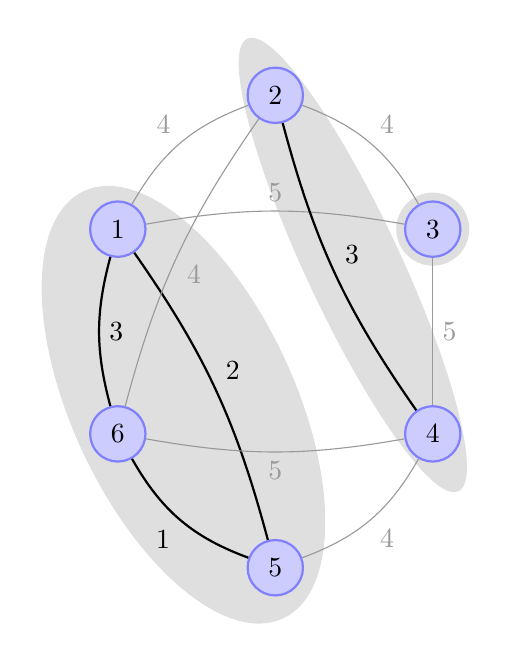
\begin{tikzpicture}
		[place1/.style={circle,draw=blue!50,fill=blue!20,thick,
inner sep=0pt,minimum size=20pt},
		place2/.style={circle,draw=green!60,fill=green!30,thick,
inner sep=0pt,minimum size=40pt},
		textstyle/.style={},
		bend angle=45,
		edgestyle/.style={-,shorten <=1pt,>=stealth’,semithick}]
		\draw[fill=gray!25,gray!25,rotate=25] (-1.45, -0.35) ellipse [x radius=40pt, y radius=85pt];
		\draw[fill=gray!25,gray!25,rotate=25] (1.25,0.35) ellipse [x radius=17pt, y radius=90pt];
		\draw[fill=gray!25,gray!25] (2.0,1.3) circle [radius=13pt];
		\node at (-2.0, 1.3) (1) [place1] {$1$};
		\node at (0.0, 3.0) (2) [place1] {$2$}
			edge [-,bend right=20,black!40] node[auto,swap] {$4$} (1);
		\node at (2.0, 1.3) (3) [place1] {$3$}
			edge [-,bend right=10,black!40] node[auto,swap] {$5$} (1)
			edge [-,bend right=20,black!40] node[auto,swap] {$4$} (2);
		\node at (2.0, -1.3) (4) [place1] {$4$}
			edge [-,bend left=10,thick] node[auto,swap] {$3$} (2)
			edge [-,bend right=0,black!40] node[auto,swap] {$5$} (3);
		\node at (0.0, -3.0) (5) [place1] {$5$}
			edge [-,bend right=20,black!40] node[auto,swap] {$4$} (4)
			edge [-,bend right=10,thick] node[auto,swap] {$2$} (1);
		\node at (-2.0, -1.3) (6) [place1] {$6$}
			edge [-,bend right=20,thick] node[auto,swap] {$1$} (5)
			edge [-,bend right=10,black!40] node[auto,swap] {$5$} (4)
			edge [-,bend left=10,black!40] node[auto,swap] {$4$} (2)
			edge [-,thick,bend left=15] node[auto,swap] {$3$} (1);
	\end{tikzpicture}
	}
	\subfigure[A possible minimum spanning tree and its connect components only considering the edges whose weight is less than 4.]{
	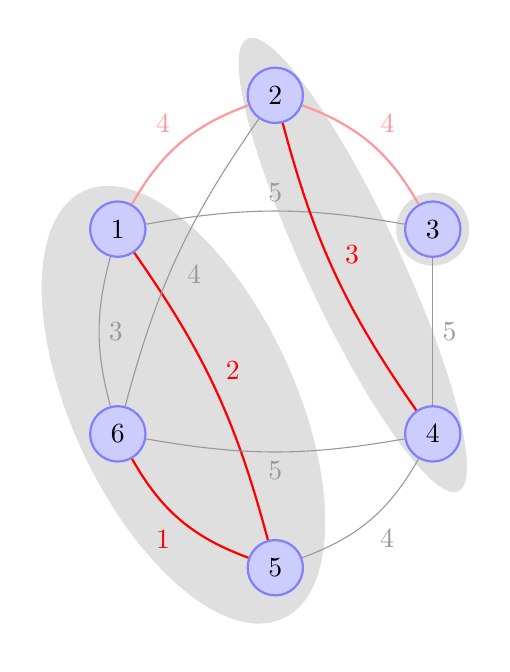
\begin{tikzpicture}
		[place1/.style={circle,draw=blue!50,fill=blue!20,thick,
inner sep=0pt,minimum size=20pt},
		place2/.style={circle,draw=green!60,fill=green!30,thick,
inner sep=0pt,minimum size=40pt},
		textstyle/.style={},
		bend angle=45,
		edgestyle/.style={-,shorten <=1pt,>=stealth’,semithick}]
		\draw[fill=gray!25,gray!25,rotate=25] (-1.45, -0.35) ellipse [x radius=40pt, y radius=85pt];
		\draw[fill=gray!25,gray!25,rotate=25] (1.25,0.35) ellipse [x radius=17pt, y radius=90pt];
		\draw[fill=gray!25,gray!25] (2.0,1.3) circle [radius=13pt];
		\node at (-2.0, 1.3) (1) [place1] {$1$};
		\node at (0.0, 3.0) (2) [place1] {$2$}
			edge [-,bend right=20,red!40,thick] node[auto,swap] {$4$} (1);
		\node at (2.0, 1.3) (3) [place1] {$3$}
			edge [-,bend right=10,black!40] node[auto,swap] {$5$} (1)
			edge [-,bend right=20,red!40,thick] node[auto,swap] {$4$} (2);
		\node at (2.0, -1.3) (4) [place1] {$4$}
			edge [-,bend left=10,red,thick] node[auto,swap] {$3$} (2)
			edge [-,bend right=0,black!40] node[auto,swap] {$5$} (3);
		\node at (0.0, -3.0) (5) [place1] {$5$}
			edge [-,bend right=20,black!40] node[auto,swap] {$4$} (4)
			edge [-,bend right=10,red,thick] node[auto,swap] {$2$} (1);
		\node at (-2.0, -1.3) (6) [place1] {$6$}
			edge [-,bend right=20,red,thick] node[auto,swap] {$1$} (5)
			edge [-,bend right=10,black!40] node[auto,swap] {$5$} (4)
			edge [-,bend left=10,black!40] node[auto,swap] {$4$} (2)
			edge [-,black!40,bend left=15] node[auto,swap] {$3$} (1);;
	\end{tikzpicture}
	}
	\subfigure[Another possible minimum spanning tree and its connect components only considering the edges whose weight is less than 4.]{
	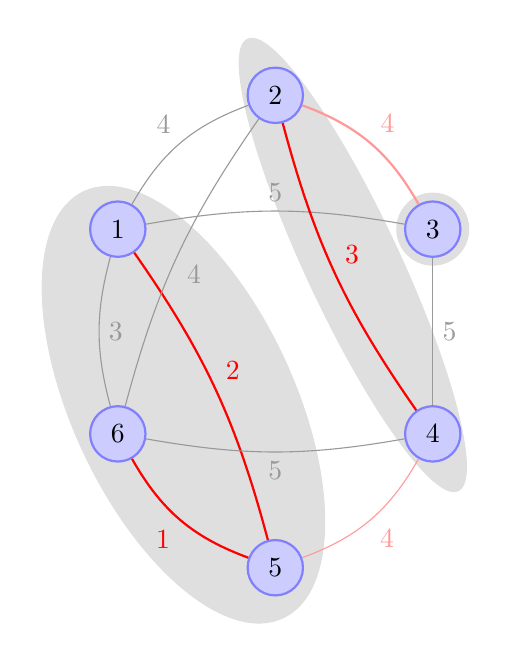
\begin{tikzpicture}
		[place1/.style={circle,draw=blue!50,fill=blue!20,thick,
inner sep=0pt,minimum size=20pt},
		place2/.style={circle,draw=green!60,fill=green!30,thick,
inner sep=0pt,minimum size=40pt},
		textstyle/.style={},
		bend angle=45,
		edgestyle/.style={-,shorten <=1pt,>=stealth’,semithick}]
		\draw[fill=gray!25,gray!25,rotate=25] (-1.45, -0.35) ellipse [x radius=40pt, y radius=85pt];
		\draw[fill=gray!25,gray!25,rotate=25] (1.25,0.35) ellipse [x radius=17pt, y radius=90pt];
		\draw[fill=gray!25,gray!25] (2.0,1.3) circle [radius=13pt];
		\node at (-2.0, 1.3) (1) [place1] {$1$};
		\node at (0.0, 3.0) (2) [place1] {$2$}
			edge [-,bend right=20,black!40] node[auto,swap] {$4$} (1);
		\node at (2.0, 1.3) (3) [place1] {$3$}
			edge [-,bend right=10,black!40] node[auto,swap] {$5$} (1)
			edge [-,bend right=20,red!40,thick] node[auto,swap] {$4$} (2);
		\node at (2.0, -1.3) (4) [place1] {$4$}
			edge [-,bend left=10,red,thick] node[auto,swap] {$3$} (2)
			edge [-,bend right=0,black!40] node[auto,swap] {$5$} (3);
		\node at (0.0, -3.0) (5) [place1] {$5$}
			edge [-,bend right=20,red!40] node[auto,swap] {$4$} (4)
			edge [-,bend right=10,red,thick] node[auto,swap] {$2$} (1);
		\node at (-2.0, -1.3) (6) [place1] {$6$}
			edge [-,bend right=20,red,thick] node[auto,swap] {$1$} (5)
			edge [-,bend right=10,black!40] node[auto,swap] {$5$} (4)
			edge [-,bend left=10,black!40] node[auto,swap] {$4$} (2)
			edge [-,black!40,bend left=15] node[auto,swap] {$3$} (1);
	\end{tikzpicture}
	}
	\caption{The illustration of the proof}
\end{figure}

	Consider $T$ itself is a subgraph of $G$, so the only case is: there exists $u, v \in V$ such that $u, v$ are not connected in $T_c$, but are connected in $G_c$. Because the $u, v$ are not connected in $T_c$, so there must be a edge $e_1$ which $w(e_1) > c$ on the path from $u$ to $v$ in $T$. This edge $e_1$ will link two components of $T$ together, let's call them $T_{1}$ and $T_{2}$.

\begin{proof}
There must exists a edge $e_2 = (x, y)$ in $G_{c}$ which $x$ is belong to $T_{1}$ and $y$ is belong to $T_{2}$.
Consider $u, v$ are connected in $G_{c}$, so there must exist a edge which can combine these two components together, otherwise $u, v$ will in two different components, and be isolated.

So, after adding this edge $e_2$ into $T$, there must form a circle in $T$. According the Cut Lemma, this edges can replace $e_1$ (for $w(e_2) \leq c < w(e_1)$), so $T$ is not the Minimum Spanning Tree of $G$, which is a contradictory. so the Lemma 3 is correct. 
\end{proof}


	\exercise{7}
	The example is illustrated below, in which we can see that no matter which minimum spanning trees we choose, the $m_3$ of each minimum spanning trees is indentical. The edges colored red are the minimum spanning tree.
\begin{figure}[H]
	\centering
	\subfigure[A possible minimum spanning tree]{
	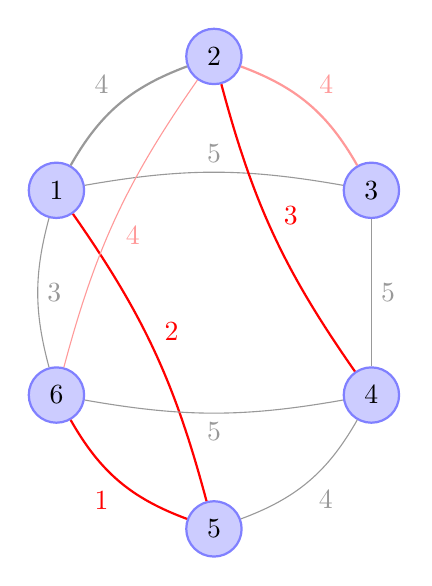
\begin{tikzpicture}
		[place1/.style={circle,draw=blue!50,fill=blue!20,thick,
inner sep=0pt,minimum size=20pt},
		place2/.style={circle,draw=green!60,fill=green!30,thick,
inner sep=0pt,minimum size=40pt},
		textstyle/.style={},
		bend angle=45,
		edgestyle/.style={-,shorten <=1pt,>=stealth’,semithick}]
		\node at (-2.0, 1.3) (1) [place1] {$1$};
		\node at (0.0, 3.0) (2) [place1] {$2$}
			edge [-,bend right=20,black!40,thick] node[auto,swap] {$4$} (1);
		\node at (2.0, 1.3) (3) [place1] {$3$}
			edge [-,bend right=10,black!40] node[auto,swap] {$5$} (1)
			edge [-,bend right=20,red!40,thick] node[auto,swap] {$4$} (2);
		\node at (2.0, -1.3) (4) [place1] {$4$}
			edge [-,bend left=10,red,thick] node[auto,swap] {$3$} (2)
			edge [-,bend right=0,black!40] node[auto,swap] {$5$} (3);
		\node at (0.0, -3.0) (5) [place1] {$5$}
			edge [-,bend right=20,black!40] node[auto,swap] {$4$} (4)
			edge [-,bend right=10,red,thick] node[auto,swap] {$2$} (1);
		\node at (-2.0, -1.3) (6) [place1] {$6$}
			edge [-,bend right=20,red,thick] node[auto,swap] {$1$} (5)
			edge [-,bend right=10,black!40] node[auto,swap] {$5$} (4)
			edge [-,bend left=10,red!40] node[auto,swap] {$4$} (2)
			edge [-,black!40,bend left=15] node[auto,swap] {$3$} (1);
	\end{tikzpicture}
	}
	\subfigure[Another possible version of the minimum spanning tree]{
	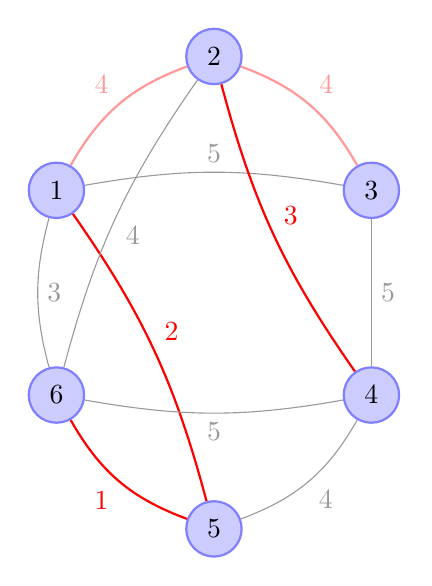
\begin{tikzpicture}
		[place1/.style={circle,draw=blue!50,fill=blue!20,thick,
inner sep=0pt,minimum size=20pt},
		place2/.style={circle,draw=green!60,fill=green!30,thick,
inner sep=0pt,minimum size=40pt},
		textstyle/.style={},
		bend angle=45,
		edgestyle/.style={-,shorten <=1pt,>=stealth’,semithick}]
		\node at (-2.0, 1.3) (1) [place1] {$1$};
		\node at (0.0, 3.0) (2) [place1] {$2$}
			edge [-,bend right=20,red!40,thick] node[auto,swap] {$4$} (1);
		\node at (2.0, 1.3) (3) [place1] {$3$}
			edge [-,bend right=10,black!40] node[auto,swap] {$5$} (1)
			edge [-,bend right=20,red!40,thick] node[auto,swap] {$4$} (2);
		\node at (2.0, -1.3) (4) [place1] {$4$}
			edge [-,bend left=10,red,thick] node[auto,swap] {$3$} (2)
			edge [-,bend right=0,black!40] node[auto,swap] {$5$} (3);
		\node at (0.0, -3.0) (5) [place1] {$5$}
			edge [-,bend right=20,black!40] node[auto,swap] {$4$} (4)
			edge [-,bend right=10,red,thick] node[auto,swap] {$2$} (1);
		\node at (-2.0, -1.3) (6) [place1] {$6$}
			edge [-,bend right=20,red,thick] node[auto,swap] {$1$} (5)
			edge [-,bend right=10,black!40] node[auto,swap] {$5$} (4)
			edge [-,bend left=10,black!40] node[auto,swap] {$4$} (2)
			edge [-,black!40,bend left=15] node[auto,swap] {$3$} (1);;
	\end{tikzpicture}
	}
	\subfigure[The remained possible minimum spanning tree]{
	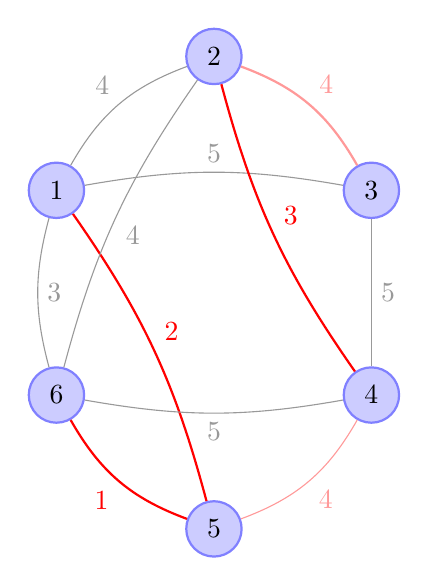
\begin{tikzpicture}
		[place1/.style={circle,draw=blue!50,fill=blue!20,thick,
inner sep=0pt,minimum size=20pt},
		place2/.style={circle,draw=green!60,fill=green!30,thick,
inner sep=0pt,minimum size=40pt},
		textstyle/.style={},
		bend angle=45,
		edgestyle/.style={-,shorten <=1pt,>=stealth’,semithick}]
		\node at (-2.0, 1.3) (1) [place1] {$1$};
		\node at (0.0, 3.0) (2) [place1] {$2$}
			edge [-,bend right=20,black!40] node[auto,swap] {$4$} (1);
		\node at (2.0, 1.3) (3) [place1] {$3$}
			edge [-,bend right=10,black!40] node[auto,swap] {$5$} (1)
			edge [-,bend right=20,red!40,thick] node[auto,swap] {$4$} (2);
		\node at (2.0, -1.3) (4) [place1] {$4$}
			edge [-,bend left=10,red,thick] node[auto,swap] {$3$} (2)
			edge [-,bend right=0,black!40] node[auto,swap] {$5$} (3);
		\node at (0.0, -3.0) (5) [place1] {$5$}
			edge [-,bend right=20,red!40] node[auto,swap] {$4$} (4)
			edge [-,bend right=10,red,thick] node[auto,swap] {$2$} (1);
		\node at (-2.0, -1.3) (6) [place1] {$6$}
			edge [-,bend right=20,red,thick] node[auto,swap] {$1$} (5)
			edge [-,bend right=10,black!40] node[auto,swap] {$5$} (4)
			edge [-,bend left=10,black!40] node[auto,swap] {$4$} (2)
			edge [-,black!40,bend left=15] node[auto,swap] {$3$} (1);
	\end{tikzpicture}
	}
	\caption{Three possible minimum spanning trees and its $m_3$}
\end{figure}


	\noindent The proof is showed below:
\begin{proof}
Because $T$ and $T'$ are two minimum spanning trees of $G$, according to Lemma 3, $T_{c}$ and $T'_{c}$ and $G_{c}$ have exactly the same components. Consider the number of components equals to $V - m_c(T)$, which $V$ is the total number of vertexs in $G$. if $m_c(T') \neq m_c(T)$, the number of components is not equal too, which is a contradictory. so $m_c(T')$ must equal to $m_c(T)$.
\end{proof}


	\exercise{8}
	Suppose that there are two different minimum spanning tree, called $T,T'$.\par

We can find the edge which belongs to only one of the minimum spanning tree and its weight is minimal.
Because no two edges of $G$ have the same weight, the above edge is unique, denoted as $e$.
(Without loss of generality, let $e$ belong to $T$)\par

By Lemma 3, we known that \[m_{c_e}\{T\} = m_{c_e}\{T'\}~\text{and}~m_{c_e - 1}\{T\} = m_{c_e - 1}\{T'\}\]
So \[m_{c_e}\{T\} -  m_{c_e - 1}\{T\} = m_{c_e}\{T'\} - m_{c_e - 1}\{T'\}\]
However, $e$ belongs to only $T$, in other word \[m_{c_e}\{T\} -  m_{c_e - 1}\{T\} = 1~\text{and}~ m_{c_e}\{T'\} - m_{c_e - 1}\{T'\} = 0\] which contradicts the equation above.\par
So, the hypothesis is wrong; that is to say $G$ has only one minimum spanning tree.


	\exercise{10}
	The two parts of the graph are independent, so we only need to caltulate the minimal spanning tree of the two parts respectively.
\begin{itemize}
	\item Left part:\par
		If we don't choose any of the parallel edges(containing three edges), we need to choose the other two edges.(1 choice).\par
		If we choose one of the parallel edges(3 choices), we only need to choose one edge from the other two edges(2 choices).\par
		In summary, we have $1 + 3 * 2 = 7$ minimal spanning trees in the left part.
	\item Right part:\par
		Using the similar method, the right part have $1 + 2 * 3 = 7$ minimal spanning trees in the right part.
	\item Combining two parts:\par
		Using Multiplication rule, we can get the total amount of the minimal spanning forests: $Num = 7 * 7 = 49$
\end {itemize}
We also justify the answer by programming(enumerating every set of the edges, and check if it can form a minimal spanning forest)

	
	\exercise{11}
		\section{Ex.11}
	Similar like Kruskal, we sort all the edges by their weight $w(e)$, then we process all the edges with the same weight in increasing order. We repeat the following works until all the edges have been processed.
	\begin{itemize}
		\item Define the smallest unprocessed edge weight as $c$. Label all the edges with $w(e)=c$ as processed.
		\item Use the given algorithm to caculate the number of spanning forests $N_c$ for a subgraph $g=(V,\{e\in E,w(e)=c\})$.
		\item According to Lemma.3, the connected components of a subgraph $G_c=(V,{e\in E,w(e)\leq c})$ are the same in spanning tree $T_c$. We can arbitrarily pick a spanning forest of $g$ and combine all the nodes in the same connected component into one node.\\
		More specificly, we define a function: $$f(u)=u'$$ where $u'$ is the node which has the smallest index in connected component containing $u$.\\ Then we modify $G$ into $G'$:
		\begin{align*}
		G'=(&\{v\in V,f(v)=v\},\\
		&\{e'=(u',v',w')|e=(u,v,w)\in E,w'=w,u'=f(u),v'=f(v),u'\neq v'\})
		\end{align*}
	\end{itemize}
	We call a combination of the spanning forests we picked in every step a solution. Finally, we get the number of solutions, as well as the number of minimum spanning trees(MST) of a weighted tree:
	$$N=\prod N_c$$
	Now we are going to show the correctness of the equality between the number of solutions and the number of MST.\par
	Since the algorithm without counting works the same as Kruskal, every solution will be an MST.\par
	Also, it's easy to see that the edges never disappear or created, so there is a bijection between the edges in the graph we compressed step by step and the edges in the orignal graph all the time. Then, for the edges with the same weight $c$ in a specific MST, we can find the step when it would be processed. Since the spanning forest we picked is arbitrary, we can choose the spanning forest which has excatly these edges we want. According to Lemma.3, those edges will always form a spanning forest with the same connected components, despite the choose of the MST. So every spanning tree is actually the same as one of the solutions.\par
	Finally, we get a bijection between $N$ solutions and all of the MST. Then the equality between the number of them holds.

\end{document}
